\documentclass[xcolor={dvipsnames,table}]{beamer}
\usepackage{epsfig,graphicx}
\usepackage{palatino}
\usepackage{fancybox}
\usepackage{relsize}
\usepackage[procnames]{listings}
\usepackage{hyperref}
\usepackage{qtree} % needed?
\usepackage{booktabs}
\usepackage{dirtree}
\usepackage[normalem]{ulem}
\usepackage{tikz}
\usetikzlibrary{arrows.meta,positioning,calc,fit,shapes.geometric,decorations.pathreplacing}


% fatter TT font
\renewcommand*\ttdefault{txtt}
% another TT, suggested by Alex
% \usepackage{inconsolata}
% \usepackage[T1]{fontenc} % needed as well?


\newcommand{\scale}{0.7}

\newcommand{\todo}[1]{{\emph{TODO: #1}}}
\newcommand{\martin}[1]{{\color{blue} Martin: #1}}
\newcommand{\abcdef}[1]{{\color{red} Author2: #1}}

% uncomment following for final submission
%\renewcommand{\todo}[1]{}
%\renewcommand{\martin}[1]{}
%\renewcommand{\author2}[1]{}

\newcommand{\code}[1]{{\texttt{#1}}}

\hypersetup{
  linkcolor  = black,
%  citecolor  = blue,
  urlcolor   = blue,
  colorlinks = true,
}

\beamertemplatenavigationsymbolsempty
\setbeamertemplate{footline}[frame number]





\newif\ifbook
\input{../shared/chisel}

% TikZ for diagrams
\usepackage{tikz}
\usetikzlibrary{positioning, arrows.meta}

% Optional visual tweaks
\tikzset{
    >=Stealth,
    every node/.style={rounded corners=2pt}
}

\title{Simple Generators}
\author{Martin Schoeberl}
\date{\today}
\institute{Technical University of Denmark\\
Embedded Systems Engineering}

\begin{document}

\begin{frame}
\titlepage
\end{frame}

\begin{frame}[fragile]{Overview}
\begin{itemize}
\item More on agile development (Scrum)
\item A bit more Scala and Chisel
\item Functional programming for generators
\item Hardware generators
\item Object-oriented hardware design
\end{itemize}
\end{frame}


\begin{frame}[fragile]{Scrum}
\begin{itemize}
\item Agile framework for development
\item Scrum is from rugby, restarting the play
\item Book  by Jeff Sutherland
\item \href{https://www.google.dk/books/edition/Scrum/RoPZCwAAQBAJ?hl=en}{Scrum
The Art of Doing Twice the Work in Half the Time}
\end{itemize}
\end{frame}


\begin{frame}[fragile]{Venn Diagram for Agile Development}
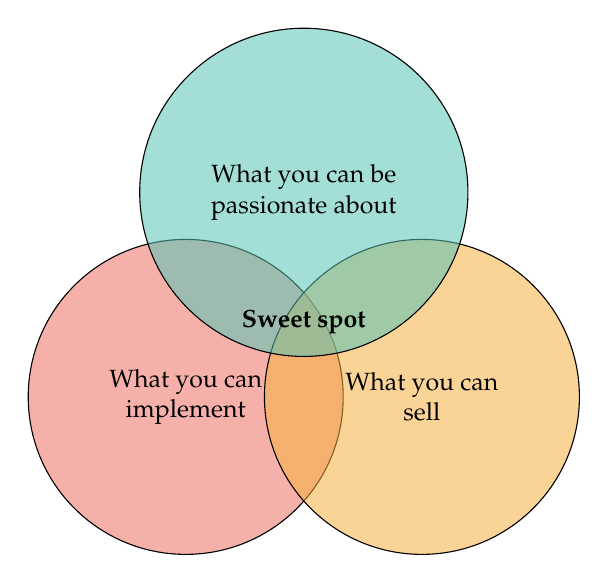
\begin{tikzpicture}
  % define pleasant colors (RGB avoids reliance on driver color sets)
  \definecolor{implColor}{RGB}{236,112,99}    % coral-ish
  \definecolor{sellColor}{RGB}{245,176,65}    % golden
  \definecolor{passionColor}{RGB}{88,196,180} % teal

  % common style for circles
  \tikzset{
    venn/.style={
      circle,
      minimum size=4cm,    % diameter ~4.8cm
      draw=black,
      fill opacity=0.55,
      text opacity=1,
      align=center,
      inner sep=6pt,
      font=\small
    }
  }

  % positions: equilateral triangle with side length = 3.0 cm
  % height = sqrt(3)/2 * side => for side=3.0 => height ~ 2.598
  \node[venn, fill=implColor]    (A) at (0,0)        {\parbox{3.2cm}{\centering What you can\\implement}};
  \node[venn, fill=sellColor]    (B) at (3.0,0)      {\parbox{3.2cm}{\centering What you can\\sell}};
  \node[venn, fill=passionColor] (C) at (1.5,2.598)  {\parbox{3.6cm}{\centering What you can be\\passionate about}};

  % optional center label (all-three overlap)
  \node at (1.5,0.95) {\small\textbf{Sweet spot}};
\end{tikzpicture}
\end{frame}

\begin{frame}[fragile]{Sprint}
\begin{itemize}
\item One or two weeks development cycle
\item Select tasks from the backlog
\item Do them during the sprint
\item Report after the sprint
\item Even show to the customer, if possible
\item Be creative about who the customer is, maybe it is me?
\end{itemize}
\end{frame}



\begin{frame}[fragile]{Things to Implement}
\begin{itemize}
\item Collect list of things in a backlog (a TODO list)
\item This is the collection for taking items for a sprint
\item Prioritise things
\item 80\% value out of 20\% feature
\item The backlog list will change
\item You will not do all things
\item Minimum viable thing first - be able to show something
\end{itemize}
\end{frame}

\begin{frame}[fragile]{More on Agile}
\begin{itemize}
\item Be open, share stuff. Best in the open, like GitHub (see my work)
\begin{itemize}
\item I have (almost) all of my work on GitHub (slides, Chisel book, code...)
\item This could be part of your CV
\end{itemize}
\item Do what you are passionate about
\begin{itemize}
\item The grade should not be what you aim for
\end{itemize}
\item Commit often
\item Demonstrate often, let us make this a weekly thing
\item Deliver value to your customer as early as possible
\item Fake it until you make it
\end{itemize}
\end{frame}

\begin{frame}[fragile]{Scrum Meetings}
\begin{itemize}
\item Have regular meetings, more often than once a week
\item Scrum is a daily standup meeting
\item Ask questions:
\begin{itemize}
\item What did you do?
\item What have you planned to do?
\item Are there roadblocks
\end{itemize}
\end{itemize}
\end{frame}

\begin{frame}[fragile]{Chisel}
\begin{itemize}
\item A hardware \emph{construction} language
\begin{itemize}
\item Constructing Hardware in a Scala Embedded Language
\item If it compiles, it is synthesizable hardware 
\item Say goodbye to your unintended latches
\end{itemize}
\item Chisel is not a high-level synthesis language
\item Single source for two targets
\begin{itemize}
\item Cycle accurate simulation (testing)
\item Verilog for synthesis
\end{itemize}
\item Embedded in Scala
\begin{itemize}
\item Full power of Scala available
\item We use Scala to write the generators
\end{itemize}
\item Developed at UC Berkeley
\end{itemize}
\end{frame}




\begin{frame}[fragile]{Chisel Example: 2-bit Counter}
\begin{verbatim}
class Counter extends Module {
  val io = IO(new Bundle {
    val out = Output(UInt(2.W))
  })
  val count = RegInit(0.U(2.W))
  count := count + 1.U
  io.out := count
}
\end{verbatim}
\end{frame}

\begin{frame}[fragile]{Example Test}
\begin{verbatim}
test(new Counter) { c =>
  c.io.out.expect(0.U)
  c.clock.step()
  c.io.out.expect(1.U)
  c.clock.step()
  c.io.out.expect(2.U)
}
\end{verbatim}
\end{frame}



\begin{frame}[fragile]{Chisel and Scala}
\begin{itemize}
\item Chisel is a library written in Scala
\begin{itemize}
\item Import the library with \code{import chisel3.\_}
\end{itemize}
\item Chisel code is Scala code
\item When it is run is \emph{generates} hardware
\begin{itemize}
\item Verilog for synthesis and simulation
\end{itemize}
\item Chisel is an embedded domain-specific language
\item Two languages in one can be a little bit confusing
\item We use Scala to program the hardware generators
\end{itemize}
\end{frame}






%\begin{frame}[fragile]{Generic Components}
%\begin{chisel}
%val c = Mux(cond, a, b)
%\end{chisel}
%\begin{itemize}
%\item This is a multiplexer
%\item Input can be any type
%\end{itemize}
%\end{frame}


\begin{frame}{Scala Summary}
\begin{itemize}
    \item Scala combines OOP and FP
    \item Programs are built from \texttt{object} + \texttt{main}
    \item \texttt{val} = immutable, \texttt{var} = mutable
    \item Strong static typing, but with type inference
    \item Functions and expressions are first-class
    \item Collections are central for data manipulation
\end{itemize}
\end{frame}

% --- Week 2: Control Structures & Functions ---
\begin{frame}[fragile]{Conditionals in Scala}
\begin{itemize}
    \item \texttt{if} is an expression that returns a value
\end{itemize}

\begin{verbatim}
val x = 10
val res = if (x > 0) "positive" else "non-positive"
println(res)   // "positive"
\end{verbatim}

\begin{itemize}
    \item \texttt{match} is similar to switch, but more powerful
\end{itemize}

\begin{verbatim}
x match {
  case 0       => "zero"
  case 1 | 2   => "one or two"
  case _       => "something else"
}
\end{verbatim}
\end{frame}

%\begin{frame}[fragile]{Functions and Recursion}
%\begin{itemize}
%    \item Functions can be recursive
%\end{itemize}
%
%\begin{verbatim}
%def fact(n: Int): Int =
%  if (n == 0) 1 else n * fact(n - 1)
%
%println(fact(5))  // 120
%
%// Tail recursion optimization
%def factTR(n: Int, acc: Int = 1): Int =
%  if (n == 0) acc else factTR(n - 1, n * acc)
%
%println(factTR(5)) // 120
%\end{verbatim}
%\end{frame}

% --- Week 3: Collections & For Comprehensions ---
\begin{frame}[fragile]{For Comprehensions}
\begin{itemize}
    \item A concise way to combine \texttt{map}, \texttt{filter}, \texttt{flatMap}
\end{itemize}

\begin{verbatim}
val nums = List(1, 2, 3, 4, 5)

// keep even numbers, square them
val result = for {
  x <- nums
  if x % 2 == 0
} yield x * x

println(result) // List(4, 16)
\end{verbatim}
\end{frame}

% --- Week 4: FP + OOP ---
\begin{frame}[fragile]{Pattern Matching}
\begin{itemize}
    \item Pattern matching decomposes values
\end{itemize}

\begin{verbatim}
def describe(x: Any): String = x match {
  case 0          => "zero"
  case true       => "true"
  case "hi"       => "a greeting"
  case i: Int     => "an integer: " + i
  case _          => "something else"
}

println(describe(42))   // "an integer: 42"
\end{verbatim}
\end{frame}

\begin{frame}[fragile]{Case Classes}
\begin{itemize}
    \item Lightweight classes with built-in pattern matching
\end{itemize}

\begin{verbatim}
case class Point(x: Int, y: Int)

val p = Point(1, 2)

// pattern match on fields
p match {
  case Point(0, 0) => println("origin")
  case Point(x, y) => println(s"($x,$y)")
}
\end{verbatim}

\begin{itemize}
    \item Case classes are nice for collecting parameters
\end{itemize}
\end{frame}

\begin{frame}[fragile]{Pure Functions}
\begin{itemize}
    \item A pure function:
    \begin{itemize}
        \item Always returns the same output for the same input
        \item Has no side effects
    \end{itemize}
\end{itemize}

\begin{verbatim}
def add(a: Int, b: Int): Int = a + b
\end{verbatim}
\begin{itemize}
    \item Combinational hardware modules are pure
    \item Side effects (state, IO, randomness) are controlled explicitly
\end{itemize}
\end{frame}



\begin{frame}[fragile]{Functions Generating Hardware}
\begin{itemize}
\item Circuits can be encapsulated in functions
\item Each \emph{function call} generates hardware
\item Simple functions can be a single line
\end{itemize}
\begin{chisel}
  def adder(v1: UInt, v2: UInt) = v1 + v2
  
  val add1 = adder(a, b)
  val add2 = adder(c, d)
\end{chisel}
\end{frame}



\begin{frame}[fragile]{Functional Abstraction}
\begin{chisel}
  def addSub(add: Bool, a: UInt, b: UInt) =
    Mux(add, a+b, a-b)

  val res = addSub(cond, a, b)
  
  def rising(d: Bool) = d && !RegNext(d)
\end{chisel}
\begin{itemize}
\item Functions for repeated pieces of logic
\item May contain state (not pure anymore)
\item Functions may return \emph{hardware}
\end{itemize}
\end{frame}

\begin{frame}[fragile]{The Counter as a Function}
\begin{itemize}
\item Longer functions in curly brackets
\item Last value is the return value
\end{itemize}
\begin{chisel}
def counter(n: UInt) = {
  
  val cntReg = RegInit(0.U(8.W))
  
  cntReg := cntReg + 1.U
  when(cntReg === n) {
    cntReg := 0.U
  }
  cntReg
}

val counter100 = counter(100.U)
\end{chisel}
\end{frame}


\begin{frame}[fragile]{Functions}
\begin{itemize}
\item Example from Patmos execute stage
\end{itemize}
\begin{chisel}
def alu(func: Bits, op1: UInt, op2: UInt): Bits = {
  val result = UInt(width = DATA_WIDTH)
  // some more lines...
  switch(func) {
    is(FUNC_ADD) { result := sum }
    is(FUNC_SUB) { result := op1 - op2 }
    is(FUNC_XOR) { result := (op1 ^ op2).toUInt }
    // some more lines
  }
  result
}
\end{chisel}
\end{frame}




\begin{frame}[fragile]{Use Functional Programming for Generators}
\shortlist{../code/fun_first.txt}
\shortlist{../code/fun_func_lit.txt}
\shortlist{../code/fun_reduce_tree.txt}
\begin{itemize}
\item This is a simple example
\item What about an arbitration tree with fair arbitration?
\end{itemize}
\end{frame}

\begin{frame}[fragile]{Functional Generation}
\begin{itemize}
\item Anonymous functions, called \emph{function literal}
\begin{chisel}
  (param) => function body
\end{chisel}
\item A function for a minimum search
\shortlist{../code/fun_min.txt}
\end{itemize}
\end{frame}




\begin{frame}[fragile]{A Simple Tester}
\begin{itemize}
\item Just using \code{println} for manual inspection
\shortlist{../code/test_bench_simple.txt}
\end{itemize}
\end{frame}


\begin{frame}[fragile]{A Test with Expect}
\begin{itemize}
\item Poke values and \code{expect} some output
\shortlist{../code/test_bench.txt}
\end{itemize}
\end{frame}

%\begin{frame}[fragile]{Testing}
%\begin{itemize}
%\item Within Chisel with a tester (= Scala program)
%\item May include waveform generation
%\item peek and poke to read and set values
%\begin{itemize}
%\item Remember the BASIC days ;-)
%\end{itemize}
%\item printf in simulation on rising edge
%\begin{chisel}
%printf("Counting %x\n", r1)
%\end{chisel}
%\end{itemize}
%\end{frame}
%
%\begin{frame}[fragile]{Testing Example}
%\shortlist{../code/test_bench_simple.txt}
%\end{frame}


\begin{frame}[fragile]{Lab 4}
\begin{itemize}
\item Write a search for the maximum circuit (with \code{treeReduce()})
\item Optional: add the generation of the index of the maximum value
\item Emit Verilog with \code{emitVerilog(new Comp())}, so you can synthesize it
\item Read the generated Verilog code
\item Code is in \href{https://github.com/schoeberl/agile-hw/tree/main/lab4}{lab4}
\end{itemize}
\end{frame}




\begin{frame}[fragile]{Scala List for Enumeration}
\begin{chisel}
  val empty :: full :: Nil = Enum(2)
\end{chisel}
\begin{itemize}
\item Can be used in wires and registers
\item Symbols for a state machine
\end{itemize}
\end{frame}

\begin{frame}[fragile]{Finite State Machine}
\begin{chisel}
  val empty :: full :: Nil = Enum(2)
  val stateReg = RegInit(empty)
  val dataReg = RegInit(0.U(size.W))

  when(stateReg === empty) {
    when(io.enq.write) {
      stateReg := full
      dataReg := io.enq.din
    }
  }.elsewhen(stateReg === full) {
    when(io.deq.read) {
      stateReg := empty
    }
  }
\end{chisel}
\begin{itemize}
\item A simple buffer for a bubble FIFO
\end{itemize}
\end{frame}

\begin{frame}[fragile]{Component Generation}
\begin{chisel}
val cores = new Array[Module](32)

for (j <- 0 until 32)
  cores(j) = Module(new CPU())
\end{chisel}
\begin{itemize}
\item Use a Scala array, or a \code{Seq}, to collect components
\item Generation with a Scala loop
\end{itemize}
\end{frame}

\begin{frame}[fragile]{Logic Generation}
\begin{itemize}
\item Read a file into a table
\begin{itemize}
\item E.g., to read in ROM content for a processor
\end{itemize}
\item Generate a truth table algorithmically
\begin{itemize}
\item E.g., generate binary to BCD translation
\end{itemize}
\item Use the full power of Scala
\end{itemize}
\begin{chisel}
val byteArray = Files.readAllBytes(Paths.get(fileName))
val arr = new Array[Bits](byteArray.length)
for (i <- 0 until byteArray.length) {
  arr(i) = Bits(byteArray(i), 8)
}
val rom = Vec[Bits](arr)
\end{chisel}
\end{frame}

\begin{frame}[fragile]{Parameterization}
\begin{chisel}
class ParamChannel(n: Int) extends Bundle {
  val data = Input(UInt(n.W))
  val ready = Output(Bool())
  val valid = Input(Bool())
}

val ch32 = new ParamChannel(32)
\end{chisel}
\begin{itemize}
\item Bundles and modules can be parametrized
\item Pass a parameter in the constructor
\end{itemize}

\end{frame}
\begin{frame}[fragile]{A Module with a Parameter}
\begin{chisel}
class ParamAdder(n: Int) extends Module {
  val io = IO(new Bundle {
    val a = Input(UInt(n.W))
    val b = Input(UInt(n.W))
    val result = Output(UInt(n.W))
  })

  val addVal = io.a + io.b
  io.result := addVal
}

val add8 = Module(new ParamAdder(8))
\end{chisel}
\begin{itemize}
\item Parameter can also be a Chisel type
\item Can also be a generic type:
\item \code{class Mod[T <: Bits](param: T) extends...}
\end{itemize}
\end{frame}

\begin{frame}[fragile]{Scala \code{for} Loop for Circuit Generation}
\begin{chisel}
val shiftReg = RegInit(0.U(8.W))

shiftReg(0) := inVal

for (i <- 1 until 8) {
  shiftReg(i) := shiftReg(i-1)
}
\end{chisel}
\begin{itemize}
\item \code{for} is Scala
\item This loop generates several connections
\item The connections are parallel hardware
\end{itemize}
\end{frame}

\begin{frame}[fragile]{Conditional Circuit Generation}
\begin{chisel}
class Base extends Module { val io = new Bundle() }
class VariantA extends Base { }
class VariantB extends Base { }

val m = if (useA) Module(new VariantA())
        else Module(new VariantB())
\end{chisel}
\begin{itemize}
\item \code{if} and \code{else} is Scala
\item \code{if} is an expression that returns a value
\begin{itemize}
\item Like ``\code{cond ? a : b;}'' in C and Java
\end{itemize}
\item This is not a hardware multiplexer
\item Decides which module to generate
\item Could even read an XML file for the configuration
\end{itemize}
\end{frame}

\begin{frame}[fragile]{Chisel has a Multiplexer}
\begin{figure}
  \includegraphics[scale=\scale]{../figures/mux}
\end{figure}
\shortlist{../code/mux.txt}
\end{frame}

\begin{frame}[fragile]{Chisel has a Multiplexer}
\begin{figure}
  \includegraphics[scale=\scale]{../figures/mux}
\end{figure}
\shortlist{../code/mux.txt}
\begin{itemize}
\item So what?
\item Wait... What type is \code{a} and \code{b}?
\begin{itemize}
\item Can be any Chisel type!
\end{itemize}
\end{itemize}
\end{frame}

\begin{frame}[fragile]{Chisel has a Generic Multiplexer}
\begin{figure}
  \includegraphics[scale=\scale]{../figures/mux}
\end{figure}
\shortlist{../code/mux.txt}
\begin{itemize}
\item SW people may not be impressed
\item They have generics since Java 1.5 in 2004
\begin{itemize}
\item \code{List<Flowers> != List<Cars>}
\end{itemize}
\end{itemize}
\end{frame}


\begin{frame}[fragile]{Generics in Hardware Construction}
\begin{itemize}
\item Chisel supports generic classes with type parameters
\item Write hardware generators independent of concrete type
\item This is a multiplexer \emph{generator}
\end{itemize}
\shortlist{../code/param_func.txt}
\end{frame}

\begin{frame}[fragile]{Put Generics Into Use}
\begin{itemize}
\item Let us implement a generic FIFO
\item Use the generic ready/valid interface from Chisel
\end{itemize}
\shortlist{../code/fifo_decoupled.txt}
\end{frame}

\begin{frame}[fragile]{Define the FIFO Interface}
\shortlist{../code/fifo_io.txt}
\begin{itemize}
\item We need enqueueing and dequeueing ports
\item Note the \code{Flipped}
\begin{itemize}
\item It switches the direction of ports
\item No more double definitions of an interface
\end{itemize}
\end{itemize}
\end{frame}

\begin{frame}[fragile]{But What FIFO Implementation?}
\begin{itemize}
\item Bubble FIFO (good for low data rate)
\item Double buffer FIFO (fast restart)
\item FIFO with memory and pointers (for larger buffers)
\begin{itemize}
\item Using flip-flops
\item Using on-chip memory
\end{itemize}
\item And some more...
\end{itemize}
\begin{itemize}
\item This calls for object-oriented \sout{programming} \emph{hardware construction}
\end{itemize}
\end{frame}

\begin{frame}[fragile]{Abstract Base Class and Concrete Extension}
\shortlist{../code/fifo_abstract.txt}
\begin{itemize}
\item May contain common code
\item Extend by concrete classes
\end{itemize}
\begin{chisel}
class BubbleFifo[T <: Data](gen: T, depth: Int) extends Fifo(gen: T, depth: Int) {
\end{chisel}
\end{frame}



\begin{frame}[fragile]{Select a Concrete FIFO Implementation}
\begin{itemize}
\item Decide at hardware generation
\item Can use all Scala/Java power for the decision
\begin{itemize}
\item Connect to a web service, get \sout{Google} Alphabet stock price, and decide on which to use ;-)
\item For sure a silly idea, but you see what is possible...
\item Developers may find clever use of the Scala/Java power
\item We could present a GUI to the user to select from
\end{itemize}
\item We use XML files parsed at hardware generation time
\item End of TCL, Python,... generated hardware
\end{itemize}
\end{frame}

\begin{frame}[fragile]{Combinational (Truth) Table Generation}
\begin{chisel}
val arr = new Array[Bits](length)
for (i <- 0 until length) {
  arr(i) = ...
}
val rom = Vec[Bits](arr)
\end{chisel}
\begin{itemize}
\item Generate a table in a Scala array
\item Use that array as input for a Chisel \code{Vec}
\item Generates a logic table at hardware construction time
\end{itemize}
\end{frame}

\begin{frame}[fragile]{Ideas for Runtime Table Generation}
\begin{itemize}
\item Assembler in Scala/Java generates the boot ROM
\item Table with a \code{sin} function
\item Binary to BCD conversion
\item Schedule table for a TDM-based network-on-chip
\item 
\item More ideas?
\end{itemize}
\end{frame}

\begin{frame}[fragile]{Test Driven Development (TDD)}
\begin{itemize}
\item Software development process
\begin{itemize}
\item Can we learn from SW development for HW design?
\end{itemize}
\item Writing the test first, then the implementation
\item Started with extreme programming
\begin{itemize}
\item Frequent releases
\item Accept change as part of the development
\end{itemize}
\item A path to \emph{Agile Hardware Development!}
\item Not used in its pure form
\begin{itemize}
\item Writing all those tests is simply considered too much work
\end{itemize}
\end{itemize}
\end{frame}

\begin{frame}[fragile]{Continuous Integration}
\begin{itemize}
\item Run your tests on each change
\item Do it also when using source control
\item GitHub Actions
\item I am doing it even for the Chisel book
\item Code that does not contain a test \emph{does not exist}
\item Chisel community does not accept a PR without a test
\end{itemize}
\end{frame}

\begin{frame}[fragile]{Testing versus Debugging}
\begin{itemize}
\item Debugging is during code development
\item Waveform and println are easy tools for debugging
\item Debugging does not help for regression tests
\item Write small test cases for regression tests
\item Keeps your code base \emph{intact} when doing changes
\item Better confidence in changes not introducing new bugs
\end{itemize}
\end{frame}


\begin{frame}[fragile]{Project}
\begin{itemize}
\item You shall start organizing into groups
\begin{itemize}
\item How shall we organize this?
\item Google Docs? DTU Learn? GitHub?
\end{itemize}
\item Think about a project
\item For inspiration, you can check Scott's students page
\item It shall be a generator, not \emph{just} hardware code
\item You shall try to explore Scrum methodology
\item Have those weekly meetings on reporting
\item We shall have some in the class
\item The report is the README.md
\end{itemize}
\end{frame}

\begin{frame}[fragile]{Lab 5}
\begin{itemize}
\item Design a component with a generic parameter
\item Emit Verilog with \code{emitVerilog(new Comp())} to read the generated code
\item README and setup is in \href{https://github.com/schoeberl/agile-hw/tree/main/lab5}{lab5}
\end{itemize}
\end{frame}


\begin{frame}[fragile]{Summary}
\begin{itemize}
\item Agile development is about changes -- it shall be fun
\item We use Scala to write hardware generators
\item Next week: guest lecture on Clash for HW generators
\end{itemize}
\end{frame}
\end{document}

\begin{frame}[fragile]{Title}
\begin{itemize}
\item abc
\end{itemize}
\end{frame}
